%
% Ziqi Tan CS 542 Class Challenge Report
%
\documentclass[a4paper,12pt]{article}
\usepackage{graphicx}
\usepackage{float}
\usepackage[english]{babel}
\usepackage[latin1]{inputenc}
\usepackage{diagbox}

\begin{document}
   \title{CS 542 Class Challenge Report \\ Image Classification of COVID-19 X-rays}
   \author{Ziqi Tan \\ E-mail: ziqi1756@bu.edu}
          
   \date{April, 18, 2020}

   \maketitle
   
   \tableofcontents
 
  \newpage
    
\section{Introduction}
In this class challenge, we will classify X-ray images. 
The data we will use has been collected by Adrian Xu, 
combining the Kaggle Chest X-ray dataset with the COVID-19 Chest X-ray dataset collected 
by Dr. Joseph Paul Cohen of the University of Montreal. 
There are two folders: 
two that will be used for a binary classification task (Task1), 
and all that will be used for multi-class classification (Task2). 
An ipython notebook template is provided for each task. 

The rest of this report will be organized as follows. 
Section 2 discusses the data preprocessing and data augmentation methods employed in these tasks.
Section 3 and 4 provide solution for task 1 and task 2, respectively. 
Each task firstly introduces the model architecture and then list the optimizer, loss function, regularization and parameters.
Finally, a t-Distributed Stochastic Neighbor Embedding (t-SNE) is used to reduce feature dimension.
In task 1, a pre-train VGG16 performs well in a binary classification problem
and it achieves a high accuracy of 95\%, but a random guess test accuracy.
Task 2 is a classification task with 4 classes. VGG16 as a good starter still achieves a high accuracy of 75\%. 
Then, ResNet50V2 architecture is taken as a competing model, which can only achieves 45\% validation accuracy 
and it gets a high test accuracy of 61.11\%.


\section{Data Preprocessing and Data Augmentation}

We could use tf.keras.preprocessing.image.ImageDataGenerator 
to preprocess the images 
and generate batches of tensor image data with real-time data augmentation.

\begin{itemize}
        \item Rescaling the images ($rescale=1.0/255$).
        \item Normalize the inputs to zero mean and divide by std of the dataset.
        \item Synthesize new images by rotating, shifting and flipping vertially and horizontally, zooming in and out and channel shift.
        \item Fraction of images reserved for validation: 0.2.
\end{itemize}

\section{Task 1 [30 points]}
Train a deep neural network model to classify normal vs. COVID-19 Xrays using the data in the folder two. Starting from a pre-trained model typically helps performance on a new task, e.g. starting with weights obtained by training on ImageNet. After training is complete, visualize features of training data by reducing their dimensionality to 2 using t-SNE. If your extracted features are good, data points representing a specific class should appear within a compact cluster. 

\subsection{Dataset}
\begin{itemize}
  \item Training set: 60 images of Covid and 70 of Normal.
  \item Test set: 9 images of Covid and 9 of Normal.
\end{itemize}



\subsection{VGG16 Architecture for task 1}
A pre-trained model VGG16 [1] has been employed in this architecture. \\

\begin{tabular}{ |p{4cm}|p{4cm}|p{4cm}|}
  \hline
  \multicolumn{3}{|c|}{Architecture} \\
  \hline
  Layer (type) & Output shape & Number of parameters \\
  \hline
  Input              & (None, 224, 224, 3)& 0 \\
  VGG16 (Model)      & (None, 7, 7, 512)  & 14714688 \\
  Flatten            & (None, 25088)      & 0   \\
  Fully connected    & (None, 256)        & 6422784 \\
  ReLu               & (None, 256)        & 0 \\
  Fully connected    & (None, 1)          & 257\\
  Sigmoid            & (None, 1)          & 0 \\
  \hline
\end{tabular}

\hfill \break

VGG16 achieves a high accuracy on image classifcation. 
The 3 fully-connected layers at the top of the VGG16 network are re-defined 
as a flatten layer, a fully-connected layer with ReLu function 
and another fully-connecte layer with Sigmoid function.
ReLu performs well in Convolutional Neural Network. 
Thus, it is chosen as the activation for the first fully-connected layer.

\begin{figure}[H]
  \centering
  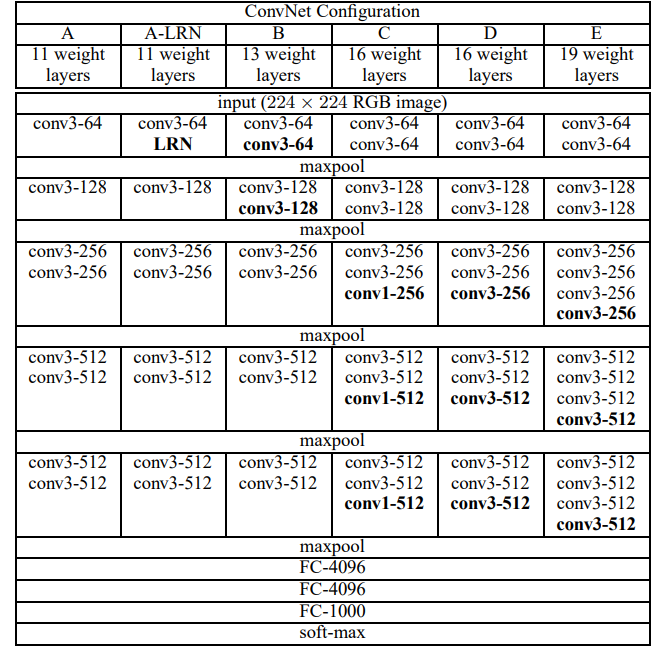
\includegraphics[width=12cm]{./images/vgg16-architecture.png}
     \caption{VGG16-Architecture [1]
             }
        \label{vgg16-architecture}
\end{figure}

\subsection{Training}
\begin{itemize}
  \item Optimizer: Adam.
  \item Loss function: tf.keras.losses.BinaryCrossentropy for binary classification problem.
  \item Epochs: 40.
  \item Batch size: 10.
\end{itemize}

\subsection{Testing}

The validation accuracy achieves around 95\%. 
However, the test accuracy is only 50\% over a test set with size of 18, 
which is a random guess in a binary classifcation problem. 
The reason may be that the training data is not enough in the first place, 
secondly, the test data may have high bias.

\subsubsection{Accuracy and Loss}
\begin{figure}[H]
  \centering
  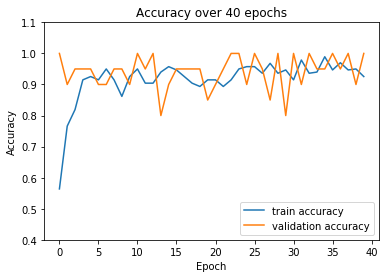
\includegraphics[width=10cm]{./images/task1-accuracy.png}
     \caption{Accuracy on training set and validation set over 40 epochs}
        \label{task1-accuracy}
\end{figure}

After 5 epochs, both train and vallidation accuracy becomes stable. 
Valication accuracy fluctuates around 95\% more drastically than train accuracy does.
The valication accuracy is approximately the same as the train accuracy, 
meaning that the model is not overfitting.

\begin{figure}[H]
  \centering
  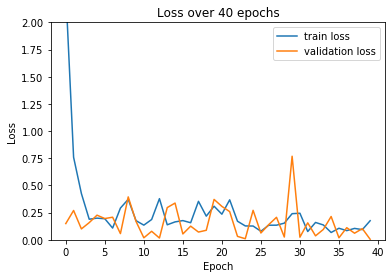
\includegraphics[width=10cm]{./images/task1-loss.png}
     \caption{Loss on trainning set and validation set over 40 epochs}
        \label{task1-loss}
\end{figure}

The train loss converges after 5 epochs, 
while the validation loss fluctuates and converges after 30 epochs.

\subsubsection{t-SNE visualizations}

We use the 130 training data to generate this feature distribution. 
The output of the first fully-connected layer with 256 neurons is taken as 
the high-dimension features. T-SEN is used to reduce 256 dimension features to 2 dimension.

\begin{figure}[H]
  \centering
  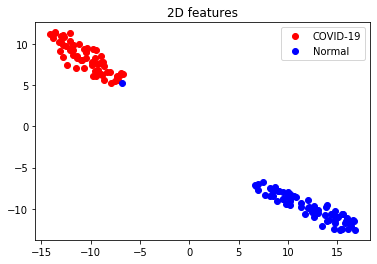
\includegraphics[width=10cm]{./images/task1-tsen.png}
     \caption{Two dimensional features on class COVID and Normal}
        \label{task1-tsen}
\end{figure}

The red points are COVID lung X-ray image and the blue are normal ones. 
The two classes is divide into two distinct clusters, 
meaning that a good classifier is established by the training of this VGG16 model.


\section{Task 2 [30 points]}
In this section you present your findings and results.
Train a deep neural network model to classify an X-ray image into one of the following classes: 
normal, COVID-19, Pneumonia-Bacterial, and Pneumonia-Viral, 
using the folder all. 
Explore at least two different model architectures for this task, eg. AlexNet vs. VGG16. 
After training is complete, visualize features of training data by reducing their dimensionality to 2 using t-SNE. 
If your extracted features are good, data points representing a specific class should appear within a compact cluster. 

\subsection{Dataset}

\begin{itemize}
  \item Training set: \\
   \begin{tabular}{ |c|c|c|c|c| }
    \hline
     & COVID-19 & Normal &  Pneumonia-Bacterial & Pneumonia-Viral\\
    \hline
    Number of images   & 9 & 9 & 9 & 9 \\
    \hline 
  \end{tabular}

  \item Test set: \\
  \begin{tabular}{ |c|c|c|c|c| }
    \hline
     & COVID-19 & Normal &  Pneumonia-Bacterial & Pneumonia-Viral\\
    \hline
    Number of images   & 60 & 70 & 70 & 70 \\
    \hline
  
  \end{tabular}
\end{itemize}


\subsection{VGG16 Architecture for task 2}
This is a subsection.

A pre-trained model VGG16 [1] has been employed in this architecture. \\


\begin{tabular}{|p{4cm}|p{4cm}|p{4cm}|}
  
  \hline
  \multicolumn{3}{|c|}{Architecture} \\
  \hline
  Layer (type) & Output shape & Number of parameters \\
  \hline
  Input              & (None, 224, 224, 3)& 0 \\
  VGG16 (Model)      & (None, 7, 7, 512)  & 14714688 \\
  Flatten            & (None, 25088)      & 0   \\
  Fully connected    & (None, 256)        & 6422784 \\
  ReLu               & (None, 256)        & 0 \\
  Fully connected    & (None, 256)        & 6422784 \\
  ReLu               & (None, 256)        & 0 \\
  Fully connected    & (None, 1)          & 257\\
  Softmax            & (None, 4)          & 0 \\
  \hline
\end{tabular}

\subsection{Training}
\begin{itemize}
  \item Optimizer: Adam.
  \item Loss function: tf.keras.losses.CategoricalCrossentropy.
  \item Epochs: 100.
  \item Regularization: dropout layers.
  \item Batch size: 10.
\end{itemize}

\subsection{Testing}
Test accuracy is 75\% and test loss is 0.7699.
\subsubsection{Accuracy and Loss}
\begin{figure}[H]
  \centering
  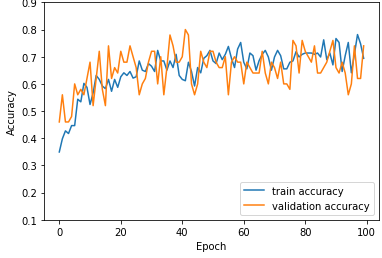
\includegraphics[width=10cm]{./images/task2-accuracy.png}
     \caption{Accuracy on training set and validation set over 100 epochs}
        \label{task2-accuracy}
\end{figure}

Train accuracy 

\begin{figure}[H]
  \centering
  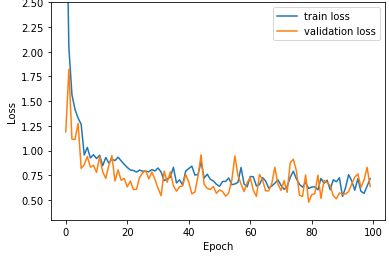
\includegraphics[width=10cm]{./images/task2-loss.png}
     \caption{Loss on trainning set and validation set over 100 epochs}
        \label{task2-loss}
\end{figure}



\subsubsection{t-SNE visualizations}
\begin{figure}[H]
  \centering
  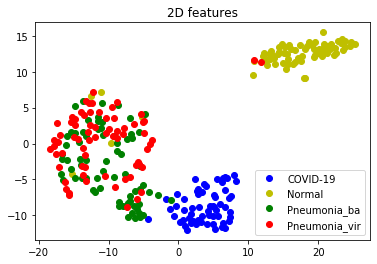
\includegraphics[width=10cm]{./images/task2-tsen.png}
     \caption{Two dimensional features on class COVID, Normal, Pneumonia\_bacterial and Pneumonia\_Viral}
        \label{task2-tsen}
\end{figure}

\subsection{ResNet50V2 Architecture for task 2}

\subsection{Training}
\subsection{Testing}

\subsubsection{Accuraccy and Loss}
\begin{figure}[H]
  \centering
  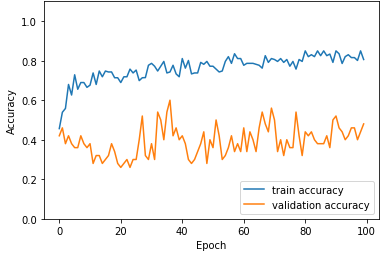
\includegraphics[width=10cm]{./images/ResNet50V2-accuracy.png}
     \caption{Accuracy on training set and validation set over 100 epochs}
        \label{task2-loss}
\end{figure}

\begin{figure}[H]
  \centering
  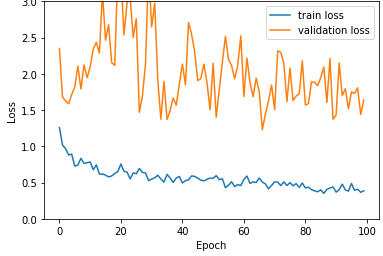
\includegraphics[width=10cm]{./images/ResNet50V2-loss.png}
     \caption{Loss on trainning set and validation set over 100 epochs}
        \label{task2-loss}
\end{figure}

\subsubsection{t-SNE visualization}
\begin{figure}[H]
  \centering
  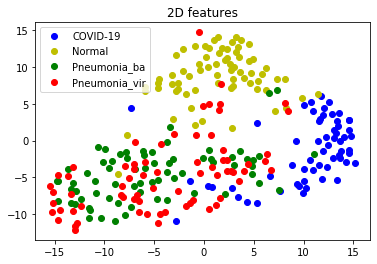
\includegraphics[width=10cm]{./images/ResNet50V2-tsen.png}
     \caption{Two dimensional features on class COVID, Normal, Pneumonia\_bacterial and Pneumonia\_Viral}
        \label{task2-tsen}
\end{figure}

\subsection{Comparasion between VGG16 and ResNet50V2}
\subsubsection{Accuraccy}
\subsubsection{Layers}
\subsubsection{Parameters}
\subsubsection{Model Complexity}

\section{Deploy Tasks on SCC Cluster [Bonus: 10 points]}

\subsection{Training time on CPU}
\begin{figure}[H]
  \centering
  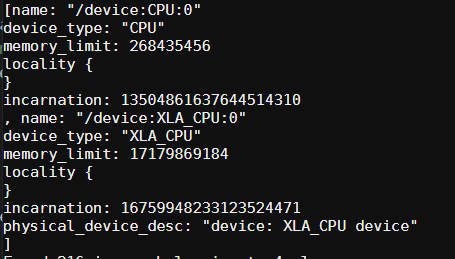
\includegraphics[width=11cm]{./images/CPU-lib.png}
     \caption{The CPU library on SCC}
        \label{CPU-lib}
\end{figure}

Print the device library. We are assigned a CPU called "device:XLA\_CPU:0".

\begin{figure}[H]
  \centering
  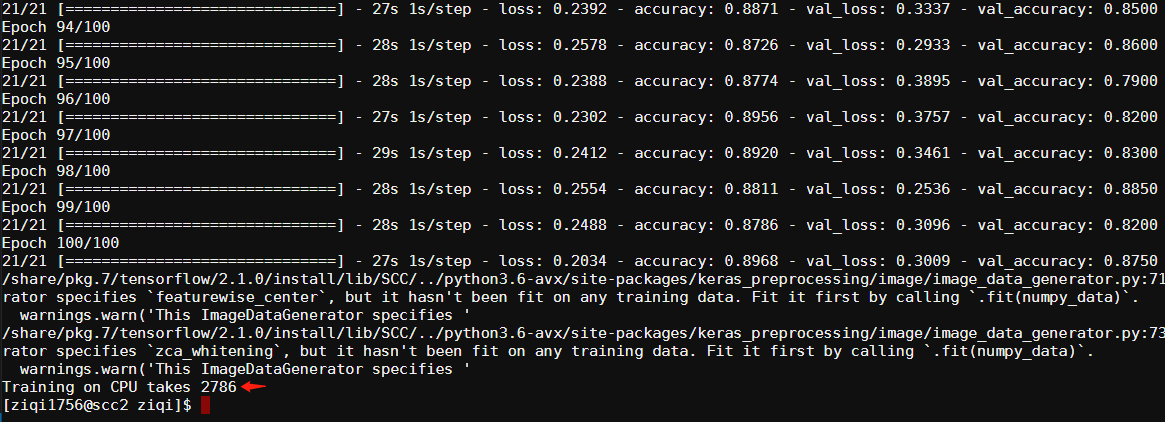
\includegraphics[width=15cm]{./images/CPU-Training-time.png}
     \caption{The time we take when training on CPU
             }
        \label{CPU-Training-time}
\end{figure}

Training on CPU takes 2786 seconds as the Fig.\ref{CPU-Training-time} shows.

\subsection{Training time on GPU}

\begin{figure}[H]
  \centering
  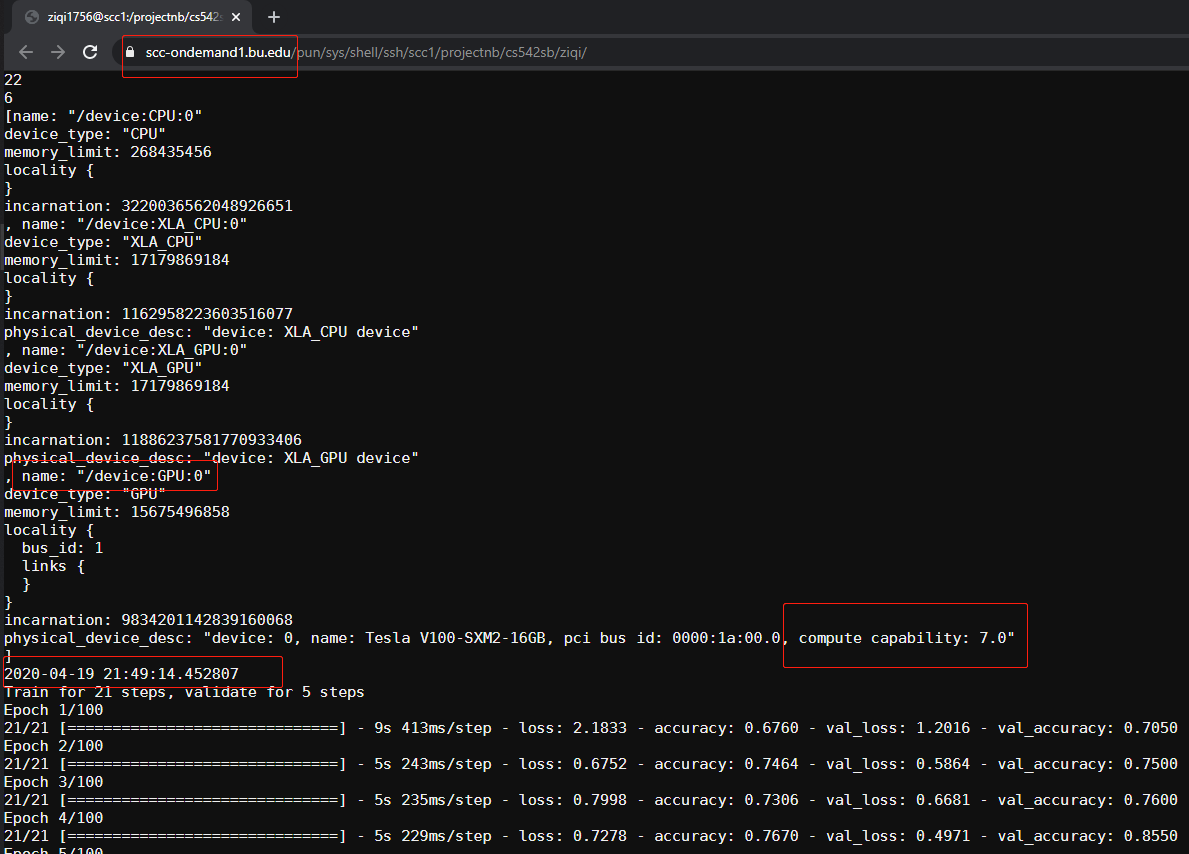
\includegraphics[width=14cm]{./images/GPU-lib.png}
     \caption{The GPU library on SCC
             }
        \label{GPU-lib}
\end{figure}

\begin{figure}[H]
  \centering
  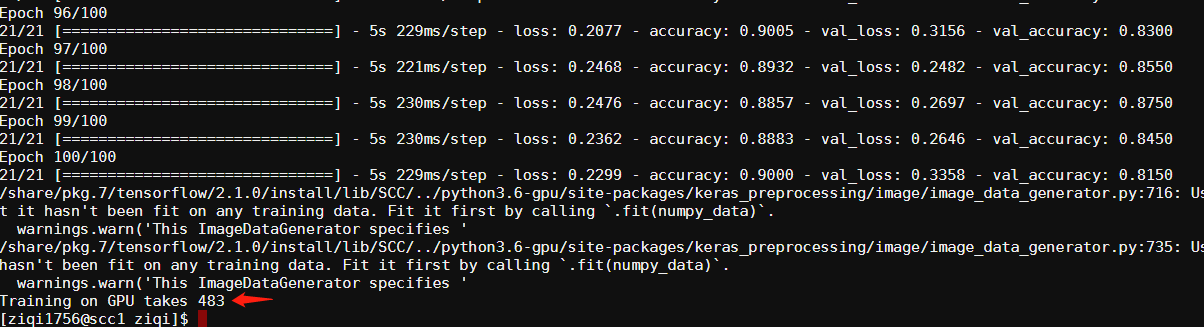
\includegraphics[width=15cm]{./images/GPU-Training-time.png}
     \caption{The time we take when training on GPU
             }
        \label{GPU-Training-time}
\end{figure}

\begin{thebibliography}{}

  \bibitem{VGG16} Karen Simonyan and Andrew Zisserman,
  Very Deep Convolutional Networks for Large-Scale Image Recognition,
  arXiv 1409.1556, cs.cv, 2014

  \bibitem{kerasCIFAR10} ResNet50V2 Documentation, https://keras.io/examples/cifar10\_resnet/

\end{thebibliography}

\end{document}

